\section{Tutorial: 4 Fotos y 1 Palabra}

En este tutorial desarrollaremos el juego \emph{4 Fotos y 1 Palabra
  (4F1P)}, que consiste en mostrar al usuario una serie de
``diapositivas'' que consisten en 4 imágenes, y un campo de texto para
que se ingrese la palabra esperada. La interfaz de usuario se muestra
en la~\Cref{fig:Slides1}.

\begin{figure}[H]
  \centering
  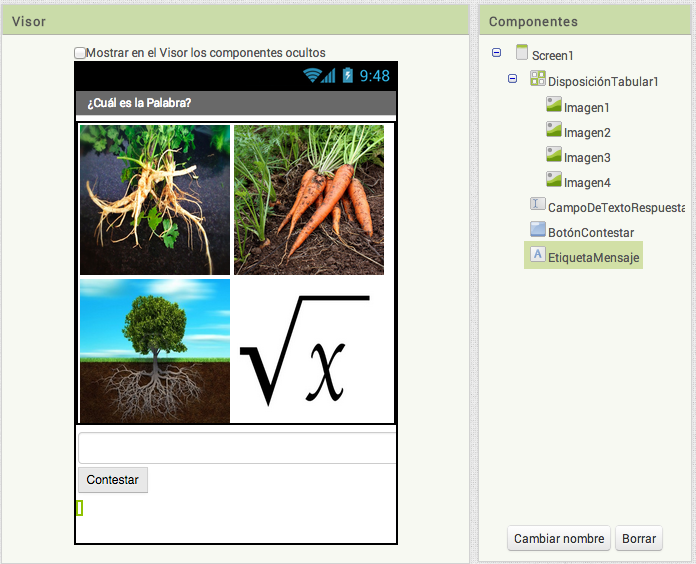
\includegraphics[scale=0.5]{Slides1}
  \caption{Interfaz de usuario \appName{4F1P}.}
  \label{fig:Slides1}
\end{figure}

En este tutorial aprenderás a recorrer una lista utilizando una
variable como \emph{índice}, para así implementar una aplicación tipo
``cuestionario'' o ``trivia''. Este tipo de aplicaciones se encuentra
tanto en juegos (como \appName{4F1P}) como en otro tipo de
aplicaciones más ``serias'' (Duolingo, Google Forms, etc.).

A continuación desarrollaremos el esqueleto de este juego, que luego
podrás completar a tu gusto.

\subsubsection*{Agregando los Componentes}

Para obtener una interfaz de usuario como la de la~\Cref{fig:Slides1}
debes utilizar los componentes que se describen en la
Tabla~\ref{tab:Slides1}

\begin{table}[H]
  \centering
  \begin{tabular}{|l|l|p{4cm}|}
    \hline
    Tipo de Componente & Nombre & Propósito\\\hline
    
    \component{DisposiciónTabular} &
    \component{DisposiciónTabular1} &
    Aquí pondrás las 4 fotos que se
    muestran para cada palabra.\\\hline

    \component{Imagen} &
    \component{Imagen1}, \component{Imagen2},
    \component{Imagen3}, \component{Imagen4} &
    Necesitas 4 componentes de imagen, que van
    dentro de las celdas de la disposición tabular.\\\hline

    \component{CampoDeTexto} &
    \component{CampoDeTextoRespuesta} &
    Aquí el usuario ingresa la palabra
    asociada a las fotos.\\\hline

    \component{Botón} &
    \component{BotónContestar} &
    Al presionar el botón la aplicación averiguará
    si la respuesta es correcta o no. Si es correcta se pasa a la
    siguiente palabra.\\\hline

    \component{Etiqueta} & 
    \component{EtiquetaMensaje} &
    Una etiqueta para mostrarle al usuario un
    mensaje cuando se equivoca.\\\hline

  \end{tabular}
  \caption{Componentes de la interfaz de usuario de \appName{4F1P}.}
  \label{tab:Slides1}
\end{table}

Una vez que ordenaste los componentes en el \designer, tienes que
configurarlos de la siguiente manera:

\begin{enumerate}

\item Cambia el \property{Título} de la pantalla a ``¿Cuál es la
  Palabra?''.

\item Configura la \component{DisposiciónTabular1} para que tenga 2 columnas y 2
  registros. Ajusta el \property{Ancho} como ``Ajustar al
  contenedor'', y el \property{Alto} en 300 pixeles.

\item Para las imágenes, ajusta su \property{Alto} y \property{Ancho}
  en 150 pixeles. Cambia la propiedad \property{Foto} de cada una de
  ellas con los textos ``raiz1.jpg'', ``raiz2.jpg'', ``raiz3.jpg'' y
  ``raiz4.jpg'', respectivamente. Los archivos los puedes encontrar en
  la carpeta \resources{ProgramaTusIdeas/Dia6}.

\item Cambia la \property{Pista} del
  \component{CampoDeTextoRespuesta1} por el texto ``Ingresa la
  palabra''.

\item Borra el texto de la \component{EtiquetaMensaje} para que esté
  vacío. Este texto lo usaremos cuando el usuario acierte o se
  equivoque en su respuesta.

\end{enumerate}

\subsubsection*{Agregando el Comportamiento}

El comportamiento de la aplicación debe ser como sigue: cuando el
usuario presiona el \component{BotónContestar}, la aplicación compara
el texto ingresado por el usuario, con la palabra esperada. Si la
respuesta coincide con la solución, se avanza a la siguiente palabra,
y se actualizan las propiedades \property{Foto} de los componentes de
imagen para que muestren la siguiente imagen en la lista.

Implementaremos este comportamiento de la siguiente manera:

\begin{enumerate}

\item Definir una variable \variable{listaPalabras} con las palabras
  que se van a mostrar en la aplicación. Además, definimos una
  variable \variable{índice} que usaremos para avanzar en la lista. En este tutorial partiremos
  con 2 palabras, como se muestra en la~\Cref{fig:Slides2}.

\begin{figure}[H]
  \centering
  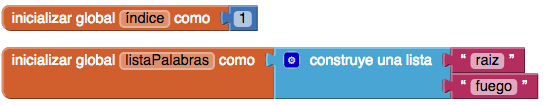
\includegraphics[scale=0.5]{Slides2}
  \caption{Lista de palabras y variable índice.}
  \label{fig:Slides2}
\end{figure}

\item Para cambiar fácilmente las fotos de los componentes de imagen,
  usaremos la convención de que los archivos serán de la forma
  ``palabra1.jpg'', ``palabra2.jpg'', ``palabra3.jpg'' y
  ``palabra4.jpg''. Esto nos permite hacer un procedimiento que
  construye los nombres de las fotos y los pone en las propiedades
  \property{Foto} de los componentes de imagen. El código se muestra
  en la~\Cref{fig:Slides3}.

\begin{figure}[H]
  \centering
  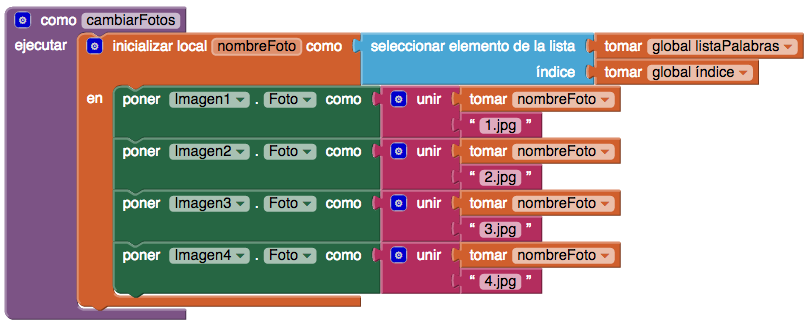
\includegraphics[scale=0.5]{Slides3}
  \caption{Procedimiento para cambiar las imágenes.}
  \label{fig:Slides3}
\end{figure}

Observa que usamos una variable local, \variable{nombreFoto}, para
evitar repetir la selección del elemento de la lista. Esto nos ayuda a
disminuir el tamaño del código. Fíjate también en que tomamos la
``palabra'' desde la \variable{listaPalabras} según el valor actual
del \variable{índice}.

\item Para procesar la respuesta del usuario debemos usar el evento
  \block{BotónContestar.Click}. Aquí debemos comparar si el texto
  ingresado por el usuario coincide con la palabra actual. Si es así,
  incrementamos el \variable{índice} y cambiamos las fotos. En caso
  contrario, mostramos un mensaje al usuario diciéndole que se
  equivocó. El código se muestra en la~\Cref{fig:Slides4}.

\begin{figure}[H]
  \centering
  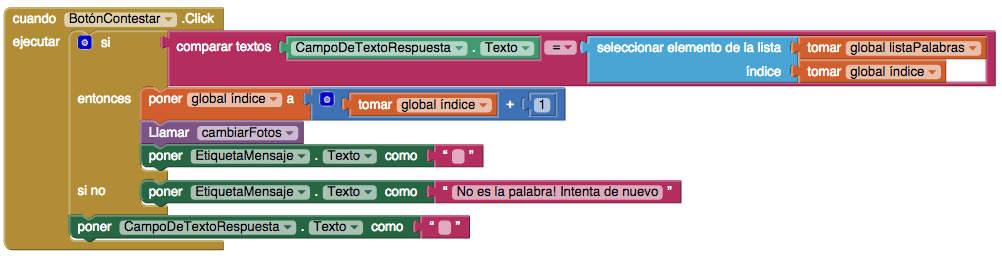
\includegraphics[scale=0.5]{Slides4}
  \caption{Verificando la respuesta del usuario.}
  \label{fig:Slides4}
\end{figure}

Para comparar los textos usamos el bloque \block{comparar textos}, que
permite ver si dos textos son iguales, o si uno es ``mayor'' o
``menor'' que otro. Para ver cuando un texto es mayor o menor se
considera el orden \emph{lexicográfico} de las letras que lo
componen. (En computación, la idea del orden lexicográfico es la misma
que la del orden alfabético, pero se usa un nombre distinto porque no
necesariamente ambos órdenes coinciden.)

\end{enumerate}

\paragraph{Prueba tu Aplicación!} Ahora ya tienes una versión inicial
de \appName{4F1P}. Prúebala en tu dispositivo: ¿qué pasa cuando te
equivocas? ¿qué pasa cuando respondes correctamente? ¿qué pasa cuando
respondes bien la segunda palabra?

\section{Desafíos de Programación}

En el tutorial desarrollaste una versión preliminar del juego
\appName{4F1P}. Sin embargo, la aplicación presenta el problema de que
se ``cae'' cuando respondes correctamente la última pregunta. El error
ocurre porque la lista de palabras tiene 2 elementos, y el código
intenta obtener el tercero---que no existe!

A la aplicación también le faltan varias cosas para ser un buen juego:
un marcador de puntaje, quizás puedas tener una cantidad de vidas, un
botón para dar pistas, etc.

Antes de mejorar esta aplicación te proponemos que revises algunos
conceptos y desafíos en una aplicación de ejemplo que es un poco más
sencilla. La aplicación se llama \appName{Slideshow} y te permite
avanzar por una lista de ``diapositivas''.

\subsection*{Ejercicios en \appName{Slideshow}}

Descarga desde \resources{ProgramaTusIdeas/Dia6} la aplicación
\appName{Slideshow} e impórtala en \AppInventor. Esta aplicación es un
poco más sencilla que \appName{4F1P}, pero tiene el mismo problema.

Tu misión es programar las siguientes variantes de la aplicación:

\begin{itemize}

\item Cambia la aplicación para que los botones ``Atrás'' y
  ``Siguiente'' le ``den la vuelta'' a la lista (es decir que se
  comporte como una \emph{lista circular}). Esto quiere decir que si
  estás en el último elemento y presionas ``Siguiente'', entonces
  vuelves al primer elemento. Además, si estás en el primer elemento y
  presionas ``Atrás'', entonces irás al último elemento.

\item Cambia la aplicación para que los botones ``Atrás'' y
  ``Siguiente'' estén deshabilitados cuando no se puedan usar. Esto
  quiere decir que si estás en el último elemento, el botón
  ``Siguiente'' debe estar deshabilitado. Además, si estás en el
  primer elemento el botón ``Atrás'' debe estar deshabilitado.

\item Agrega a la aplicación un botón ``Empezar'' que haga que las
  diapositivas avancen automáticamente cada 5 segundos.

\end{itemize}

\subsection*{Personaliza y Crea Tus Propias Aplicaciones}

Puedes extender y mejorar las aplicaciones \appName{Slideshow} y
\appName{4F1P}. Además, te proponemos que desarrolles otra aplicación
\appName{Identifica a tus Compañeros}. En esta aplicación puedes
mostrar la foto de tus compañeros y debes escribir su nombre. Te damos
algunas ideas adicionales:

\begin{itemize}

\item Utiliza otro recursos multimedia como videos y sonidos. Por
  ejemplo, en \appName{Identifica a tus Compañeros} puedes alternar
  entre fotos y grabaciones de voz. Si usas más archivos de sonidos
  puedes crear una aplicación para identificar canciones o melodías!

\item El código para comparar las respuestas es muy estricto, por
  ejemplo ``Raiz'' y ``raiz'' no se consideran iguales porque una
  letra es mayúscula y la otra no. Soluciona esto mediante una
  \emph{normalización} del texto ingresado por el usuario, usando
  bloques de la sección ``Texto''. Por ejemplo, puedes pasar el texto
  a minúsculas y remover todos los acentos.

\item Crea una aplicación con preguntas de selección múltiple. Vas a
  tener que almacenar las posibles respuestas dentro de listas, por lo
  que tendras que manejar una lista de listas. Utiliza el componente
  \component{SelectorDeLista} para que el usuario elija una respuesta.

\item Combinando lo anterior, puedes crear una aplicación al estilo
  \emph{Quién Quiere ser Millonario}, incorporar comodines, etc.

\end{itemize}

\section{Material de Apoyo}

\subsection*{Navegación de una Lista}

¿Cómo se puede recorrer una lista con información? Ya sabemos que
\AppInventor provee el bloque \block{por cada ...} que permite
procesar todos los elementos de una lista, uno por uno; pero que
esencialmente los procesa todos a la vez. ¿Qué pasa si tienes una
aplicación como una trivia o un pase de diapositivas, en la cual el
usuario controla el movimiento a través de la lista? Para programar
este comportamiento, necesitas usar una varíable como \emph{índice}
para registrar tu posición en la lista. Revisa los siguientes
ejemplos.

\paragraph{Ejemplo: ¿Cómo creas un pase de diapositivas donde el
  usuario presiona un botón para ver la siguiente foto?}

En este ejemplo, el usuario presiona un botón para avanzar en la
secuencia de diapositivas que contienen fotos. Las imágenes
corresponden a los archivos \mediafile{foto1.jpg},
\mediafile{foto2.jpg} y \mediafile{foto3.jpg}, las cuales han sido
subidas a la aplicación. La~\Cref{fig:List1} muestra el código de la
aplicación.

\begin{figure}[H]
  \centering
  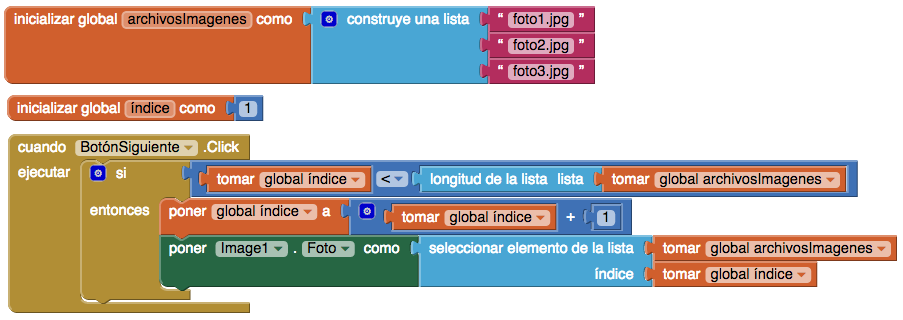
\includegraphics[scale=0.5]{List1}  
  \caption{Código aplicación para pase de diapositivas.}
  \label{fig:List1}
\end{figure}

La variable \variable{índice} se define para mantener un registro de
la posición de la figura actual que el usuario está viendo. Cuando el
usuario presiona ``Siguiente'', se averigua si el índice ha ido muy
lejos (más allá del largo de la lista). Si el índice es menor que el
largo de la lista, que en este caso es 3, entonces el índice se
incrementa y se pone la siguiente imagen de la lista en la propiedad
\property{Imagen1.Foto}.

Veamos paso a paso este ejemplo. Asume que \mediafile{foto1.jpg} se
muestra cuando se inicia la aplicación. Cuando el usuario presiona
``Siguiente'', se revisa el \variable{índice} y efectivamente es menor
que el largo de la lista (sabemos que $1 < 3$). Por lo tanto se
incrementa el \variable{índice} desde su valor inicial 1, al valor 2;
y se selecciona y muestra la \mediafile{foto2.jpg}.

La próxima vez que el usuario presiona ``Siguiente'', el índice es 2
por lo que sigue siendo menor que 3, así que se incrementa su valor a
3 y se muestra la tercera foto, \mediafile{foto3.jpg}.

Cuando se presiona otra vez ``Siguiente'', el \variable{índice} vale 3
por lo tanto el chequeo ($3 < 3$ no es verdad) falla. Por lo tanto los
bloques dentro del condicional no se ejecutan---y nada pasa. De hecho,
el usuario puede seguir presionando ``Siguiente'' mil veces, sin
efecto alguno.

\paragraph{Ejemplo: ¿Cómo agregar un botón ``Atrás'' para mostrar las
  diapositivas anteriores?}

El código de este ejemplo, que se ve en la~\Cref{fig:List2} es similar
al botón ``Siguiente'' anterior, pero ahora el \variable{índice} se
disminuye para volver a la diapositiva anterior. En este caso la
condición chequea si el \variable{índice} es mayor que 1; porque si ya
es 1, ya se está mostrando la primera foto y no es posible ir más
atrás.

\begin{figure}[H]
  \centering
  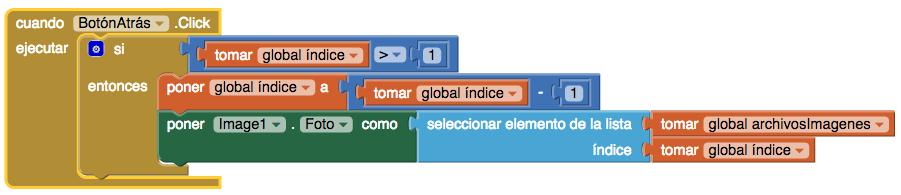
\includegraphics[scale=0.5]{List2}  
  \caption{Código para botón ``Atrás''.}
  \label{fig:List2}
\end{figure}

\paragraph{Ejemplo: ¿Cómo comenzar nuevamente las diapositivas una vez
llegado al final?}

En el ejemplo de la~\Cref{fig:List3}, cuando el usuario presiona
``Siguiente'' cuando se está mostrando la última diapositiva, el
\variable{índice} se pone como 1 nuevamente, lo que hace que se
``reinicie'' el pase de diapositivas. El bloque \block{poner
  Imagen1.Foto} ahora está afuera del bloque \block{si-sino} por lo
tanto siempre se mostrará una foto diferente cuando el usuario
presiona ``Siguiente''.

\begin{figure}[H]
  \centering
  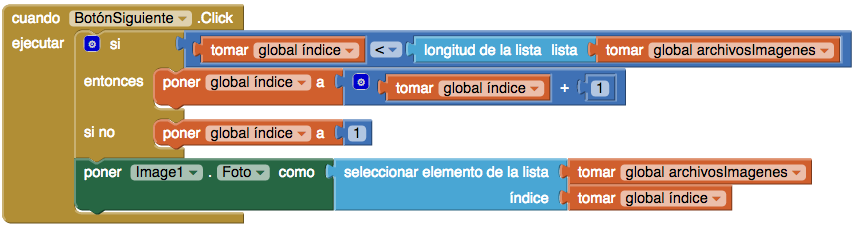
\includegraphics[scale=0.5]{List3}  
  \caption{Código para reiniciar una vez terminado el recorrido.}
  \label{fig:List3}
\end{figure}
